

\chapter{Introducción}
El objetivo de esta tesis es encontrar soluciones periódicas a ecuaciones diferenciales con medidas o MDE\index{MDE}, las cuales se pueden definir de manera general como 
	\begin{equation*}
	\left\lbrace \begin{array}{l} \label{eq:problema A}
		d\varphi=F(t,\varphi(t))\;d \mu\\
		\varphi(0)-\varphi(T)=0,
	\end{array}\right. \tag{${MDE}$}
\end{equation*}
donde $F:[0,T]\times\rr^n\to\rr^{n\times m}$ es una función con valores matriciales, $\mu$ es una medida vectorial con valores en $\rr^m$, $\varphi:[0,T]\to \rr^n$ es una función de variación acotada  y $d\varphi$ es la medida vectorial Lebesgue-Stieltjes asociada a $\varphi$.

 Las MDE intervienen en modelos no suaves de varias ramas de la ciencia, como los modelos que describen el movimiento de moléculas en gases ideales hasta el análisis de la dinámica \highlight[comment={No quedará mejor expresado si decimos ``de los impactos de una pelota en una raqueta''? }]{de la pelota raqueta}. En  física e ingeniería mecánica intervienen en el estudio de materia granular y \reversemarginpar\highlight[comment={Qué son los morores de arena?. Lo googlie y me parece que son como filtros de pileta. No los denominaremos de otra forma en argentina?}]{ motores de arena}; en la robótica, se usan para estudiar impactos en las articulaciones (ver \cite{Brogliato} y \cite{ALeonov}). Un caso particular donde intervienen MDE es \replaced{aquel}{aquél} dado por los modelos impulsivos, ver \cite{Bainov},\cite{Bainov_2} y \cite{Lakshmikan}. Por ejemplo, en los sistemas mecánicos se puede pensar que el impacto entre dos cuerpos es un fenómeno de muy corta duración que implica un cambio brusco en la dinámica de los cuerpos. Es por eso que,\normalmarginpar\comment{Para mi no iría coma aquí} se suele representar \textcolor{red} {a}\comment{Está en rojo} los impactos como fuerzas muy grandes que actúan en un tiempo infinitamente corto. Supongamos que durante el impacto o colisión actúa una fuerza $F$ y que este ocurre en un intervalo $[t_0,t_0+\Delta t]$, entonces el cambio en la cantidad de movimiento es igual al impulso que genera la fuerza \index{impulso} \cite{Serway}, o sea
$$I=\Delta p=\int_{t_0}^{t_0+\Delta t}F(s)ds.$$
Si suponemos que la fuerza actúa\comment{Le buscaría un sinónimo a actúa, está muy repetido} en un intervalo muy chico, tanto que podemos decir que es instantánea, entonces el impulso es
    \begin{equation*}
        I=\lim_{\Delta t \to 0}\int_{t_0}^{t_0+\Delta t}F(s) ds. 
    \end{equation*}
    \newpage
Para que el impulso $I$ sea distinto de cero, $F(\cdot)$ debe tomar valores \highlight[comment={ No lo diría así, en realidad hacer infinito a $F$ tampoco arreglaría nada. ¿Qué te aparece decir lo siguiente? Si en la integral tuviesemos una función común integrada respecto a la medida de lebesgue el límite sería cero por la absoluta continuidad de la integral. Por eso necesitamos integrar respecto a medidas que no sea absolutamente continuas respecto a la medida de lebesgue}]{infinitos} ya que la medida de Lebesgue del intervalo tiende a cero. Por eso, es conveniente tomar a la fuerza como una medida de Dirac concentrada en el tiempo $t_0$ (la cual expresaremos como $\delta_{t_0}$\index[Simbolo]{$\delta_{t_0}$}) y de magnitud $I$, es decir $F(t)=I\delta_{t_0}$. A este tipo de fuerza se la  denomina fuerza impulsiva\index{fuerza impulsiva}.

{\color{blue} Otra fuente de problemas con medidas son los problemas de control. Podes agregar una breve mención sobre eso (podes sacar una idea del primer párrafo en el prefacio de \cite{S.T.Zavalishchin}). También agregaría algo asi: <<Más allá de las aplicaciones, los problemas de ecuaciones diferenciales con medidas son, desde el punto de vista exclusivamente matemático, una generalización natural de las ecuaciones diferenciales ordinarias y a nuestro juicio este hecho ya justificaría su estudio. Varias teorías de integración han sido utilizadas para abordar problemas como los planteados en esta tesis, a saber integrales de Lebesgue-Stieltjes, Perron-Stieltjes, Kurzweil-Henstock (ver por ejemplo    \cite{S.Schwabik320,JaroslavKurzweil1411,StefanSchwabik75,EveraldoM.Bonotto420}).>>}


\begin{example} \label{ejemplo1}
    Supongamos que un cuerpo de masa $m$ se mueve con velocidad constante sobre una recta, y se somete a impulsos $I_k$ en los instantes $t_k$. Como el impulso es el cambio en la cantidad de movimiento (\cite{Serway}), entonces $I_k=mv(t_k^+)-mv(t_k^-)$. Podemos decir que si el movimiento del cuerpo está dado por la función $x(t)$, entonces cumple la siguiente ecuación 
    \begin{equation}
	\left\lbrace \begin{array}{lll} 
		\label{eq:imp}
        x''(t)=0 & \text{si }& t\neq t_k,\\
		x'(t_k^+)-x'(t_k^-)=\dfrac{I_k} {m} & \text{ para }& k=1,..,r.\tag{${PI}$}
	\end{array}\right. 
\end{equation}
Si ahora consideramos la fuerza impulsiva $F(t)=\displaystyle\sum_{k=1}^r I_k\delta_{t_k},$ entonces podemos \deleted{puedo} escribir el problema impulsivo \ref{eq:imp} como una \ref{eq:problema A}
$$d(x'(t))=\sum_{k=1}^r\dfrac{I_k}{m}\delta_{t_k}\textrm{\todo{No escribiría $d(x'(t))$ porque reigurosamente hablando sería el diferencial de una constante, sería $0$. Pondría simplemente $dx'$ (fijate que en el miembro de la derecha no hay $t$, tampoco te hace falta a la izquierda}}$$
\end{example}
\textcolor{blue}{
Los modelos impulsivos intervienen en otras ciencias, además de física o matemática, como por ejemplo en biología.}
 

\begin{example}\label{ejemplo2}
\textcolor{blue}{La ecuación 
\begin{equation}\label{ec:biomasa}
    x'=rx\left(1-\dfrac{x}{K}\right),
\end{equation}
describe los cambios en el número de individuos $x(t)$ en una población aislada, de alguna especie biológica con una taza de reproducción $r$, en un ambiente estacionario con una capacidad máxima de $K$. Para ser más precisos, supondremos que $x(t)$ es la cantidad de biomasa de una determinada especie de microorganismo cultivado en un biorreactor. Los efectos externos sobre el desarrollo de la especie pueden provocar saltos en la cantidad de biomasa $x(t)$. Esto es posible, por ejemplo, con una sola extracción de una parte de la biomasa o con la introducción de una cantidad adicional de biomasa. Los  efectos externos en el momento $t=t_k$ generan que la  cantidad de biomasa sufra un incremento, es decir 
$$I_k=\Delta x(t_k)=x(t_k^+)-x(t_k^-).$$
Como en el ejemplo anterior, este tipo de problemas puede ser descripto usando MDE.
En este caso, tendríamos una parte de la ecuación no impulsiva o suave $f(t,x)=rx\left(1-\dfrac{x}{K}\right)$, en donde actuaría la medida de Lebesgue (usaremos el símbolo $d\lambda$, para diferenciarla de otras medidas\comment{ya está dicho}) y otra parte impulsiva o no suave donde estaría el impulso $I_k$ con la medida de Dirac.
\begin{equation*}
    d(x)=rx\left(1-\dfrac{x}{K}\right)d\lambda +g(x)d\delta_{t_k}.
\end{equation*}}
\end{example}



%\begin{example}
%    \begin{equation*}
%	\left\lbrace \begin{array}{lcr} 
%		x'=1+x^2,\\
%        x(0)=0\\
%		\Delta x(t_k)=-1 &t_k=\frac{k\pi}{4}&k=1,2,....
%	\end{array}\right. 
%\end{equation*}
%Si notamos $d\lambda$ a la medida de Lebesgue \index[Simbolo]{$d\lambda$}, el problema anterior se puede expresar como una MDE de la siguiente manera
%\begin{equation*}
%	\left\lbrace \begin{array}{lcr} 
%		x'=1+x^2 \;d\lambda-\displaystyle\sum_{k=1}^{\infty}d\delta_{t_k}(t),\\
%        x(0)=0.\\
	%	\end{array}\right. 
%\end{equation*}
%La solución es $x(t)=\tan(t-\frac{k\pi}{4})$ donde $\frac{k\pi}{4}\leq %t <\frac{(k+1)\pi}{4}$, y tiene período $\pi/4$.
%\begin{figure}[h!]
%    \centering
%    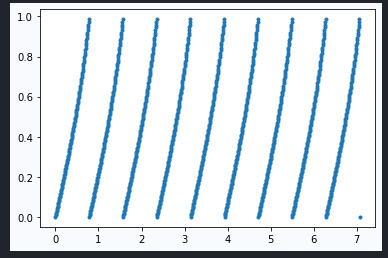
\includegraphics[width=0.7\linewidth]{img.ejem1.png}
%    \caption{}
%    \label{fig:ejemple1}
%\end{figure}



%\end{example}

Las ecuaciones impulsivas se pueden generalizar para casos donde actúan fuerzas no impulsivas $f(t,x)$ y/o  donde se aplique una cantidad infinita de impulso. Un caso general se puede ver en \cite{Bainov}, está dado por
	\begin{equation*}
		\left\lbrace \begin{array}{l}
			x''=f(t,x(t)) \; \text{si }\; t\neq t_k\\
			 x'(t_k^+)-x'(t_k^-)=I_k \; \text{ donde }\; k=1,2,....,
		\end{array}\right. 
	\end{equation*}
donde, como vimos en el ejemplo \ref{ejemplo1}, se pude pensar a los impulsos como suma de deltas de Dirac concentradas en $t_k$ y 
empleando la medida de Lebesgue $d\lambda$.\index[Simbolo]{$d\lambda$}
$$dx'=f(t,x(t)) d\lambda +\sum_{k=1}^{\infty}I_k\;d\delta_{t_k}$$

Para resolver ecuaciones como \eqref{eq:problema A}, usaremos una 
metodología inspirada 
en   la sección 1.3 del
libro de Pablo Amster.
Allí utiliza el método Shooting para hallar soluciones al problema de contorno periódico 

	\begin{equation*}
		\left\lbrace \begin{array}{l}
			u'=f(t,u(t))\\
			u(0)-u(T)=0,
		\end{array}\right. 
	\end{equation*}
donde $f$ es una función continua y Lipschitz en la segunda variable $u\in\rr^2$.  La idea que propone Pablo Amster \replaced{consiste}{conciste} en buscar una solución $u_\alpha$ al problema de valores iniciales 
	\begin{equation*}
	\left\lbrace \begin{array}{lcl}
		u'&=&f(t,u(t))\\
		u(0)&=&\alpha,
	\end{array}\right. 
\end{equation*}
y buscar un valor de $\alpha\in\rr^2$ tal que $u_\lambda(T)=\alpha$. Es decir,
$u_\alpha$ no es otra cosa que  un punto fijo del operador de Poíncare\index{operador de Poíncare} $P:\rr^2\to \rr^2$, definido como $P(\alpha)=u_\alpha(T)$. Bajo ciertas condiciones, aplicando el Teorema de Brouwer \cite{Amster} al operador podemos asegurar la existencia de la solución al problema periódico. 

En el capítulo 2 haremos una breve introducción a la medida de Lebesgue-Stieltjes y sus propiedades. 
En el capitulo 3 se encuentran los resultados principales de este trabajo de tesis. En la sección 3.1 vamos a ver como transformar el problema \eqref{eq:problema A} con medidas vectoriales a uno donde intervenga una sola medida positiva. En la sección 3.2 estableceremos las condiciones para la existencia de soluciones al problema de valores iniciales y su continuación a intervalos máximos. En la sección 3.3 enunciaremos y demostraremos una versión del teorema de Gronwall que hemos obtenido para medidas de Borel. A partir de este teorema, probaremos  la continuidad del operador de Poincaré y finalmente podremos usar el Teorema Brouwer y 
hallar un punto fijo para el operador de Poincaré.  









